\clearpage
\cleardoublepage

\chapter{Approach}
\label{chap:approach}
In  \autoref{chap:related_work} I discussed different architectures and convolutions on non-Euclidean spaces, specifically spherical CNN which brings closer the
representation of geospatial data closer to the actual representation of the Earth. Regardless of the advances being done in the geometric machine learning,
most of the GIS systems are in use of map projections for geospatial data for the analysis. In particular, specific types of map projections are only used for
the analysis of the geospatial data in the GIS systems. The GIS systems are only focusing on cylindrical projections and over looking the errors generated by
the distorted projections. Even though there are numerous projections in the literature, a thorough investigation of the different types of map projections is still
needed which could bring out the potential for the representation of the geospatial data on the global level. Map projections employ an approximation of the true form
of the geoid using an ellipsoid. This has motivated our investigation into the different types of map projections for geospatial analysis.

\begin{figure}[h]
    \centering
    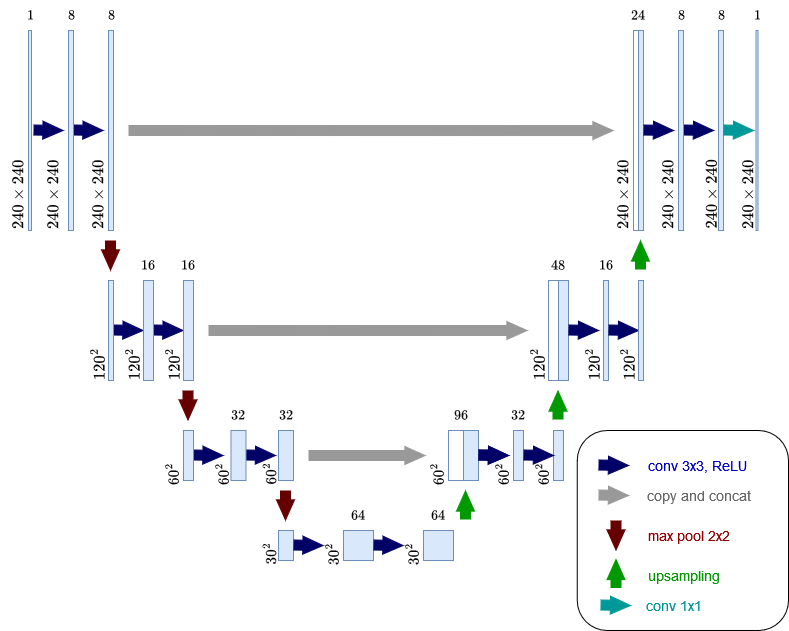
\includegraphics[width=1.0\linewidth]{figures/chapter-5/my_unet.png}
    \caption{U-Net architecture for experimentation }
    \label{fig:self-unet}
\end{figure}

Map projections are planer in nature, to capture the spatial correlation on the projected geospatial data, I utilized the power of convolutional neural networks.
In specific I used the U-NET \cite{ronneberger2015unet}  based architecture to understand the effects on 2D convolutions following \cite{trebing2021smaatunet}, to generate projected precipitation data on the global scale by giving the geopotential height projected data as input to the U-Net model.

\section{Architecture}
For this purpose, I defined a shallow U-Net \textbf{architecture}, with four contraction blocks which contains two convolutional layers with rectified linear unit (\textbf{ReLU})
as activation function, with zero-padding and kernel of size (\textbf{3x3}), for contracting the feature maps max pooling layer with pool size (\textbf{2x2}) is used after the two
convolutional layers.
After the contraction blocks the expansion block are introduced in the architecture with up sampling layers with \textbf{interpolation} strategy of the nearest neighbors is used
and followed by two convolutional layers with same settings as in the contracting path of the model.
The last layer in which the network is generating the map projected precipitation rasters, a 2D convolutional layer is used by kernel size  \textbf{(1x1)}.

The main feature in the U-Net architecture is that the feature maps from the encoder part of the model (left hand side) shown in the figure ~\ref{fig:self-unet} are concatenated to the decoder part of the model (right hand side).
This concatenation enhances the reconstruction of the output by joining the hierarchically learned features at each encoder's convolutional block of the network. This could be
understood as the convolutional neural networks make sense of the features in an hierarchical manner by passing feature maps and performing convolutions at deeper levels,
learning the primitive features at the upper level and learning the fine grained features are the deeper level. The reconstruction of the precipitation raster in the decoder
part happens in a bottom up fashion facilitated by the concatenation of the features maps of the encoder part of the network. Figure ~\ref{fig:self-unet} depicts the complete architecture.

\section{Hyper Parameters}
\begin{itemize}
    \item The learning rate for the training of the loss function is $\eta = 0.001$, the learning rate was kept same for all the experiments regarding different map projection types to see only the effects of the convolutions on the map projections.
    \item \textbf{Adam optimization} is used for the boosting the training of the model.
\end{itemize}

\begin{figure}[h]
    \centering
    \begin{minipage}{0.45\textwidth}
        \centering
        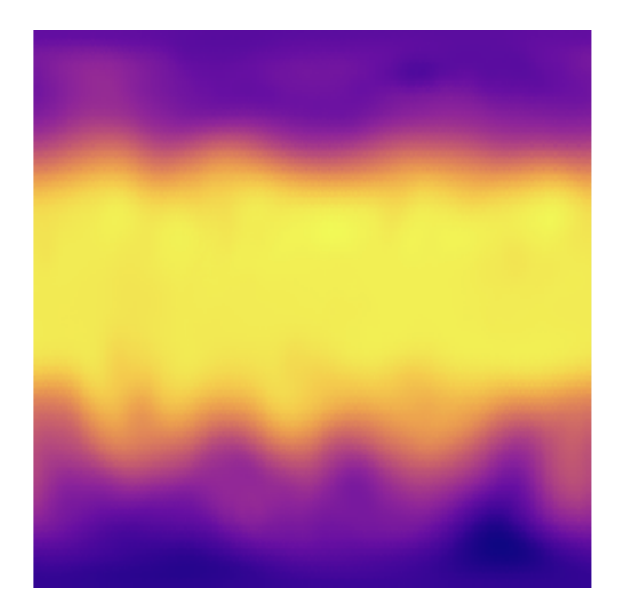
\includegraphics[width=0.9\linewidth]{figures/chapter-5/plate_caree_geopoth_raster.png}
        \caption{ Geopotential height raster data as Plate-Carrée projection}
        \label{fig:plate_geopoth_raster}
    \end{minipage}\hfill
    \begin{minipage}{0.45\textwidth}
        \centering
        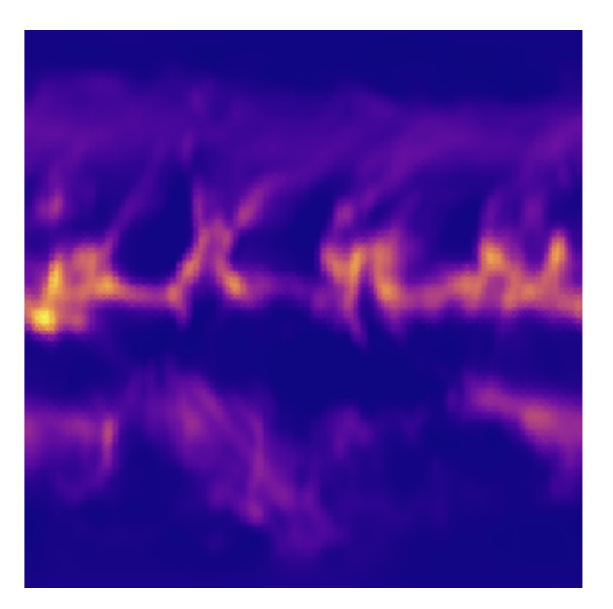
\includegraphics[width=0.9\linewidth]{figures/chapter-5/plate_caree_prect_raster.png}
        \caption{Precipitation raster data as Plate-Carrée projection}
        \label{fig:plate_prect_raster}
    \end{minipage}\hfill
\end{figure}

\newpage

\section{Training Process}

For the setting of our experiments, I considered the prediction of the precipitation on the global level on the basis of geopotential height as a regression problem. For this reason I selected mean squared error (MSE) as a loss function for training the model.

Mean Squared Error is defined as:

\begin{gather*}
    MSE = \dfrac{1}{n}\sum_{1 = 1}^{n}(Y_i-\hat{Y}_i )^2
\end{gather*}

The training process of models is depending on the preprocessing of the geospatial data, where the original data is converted to rasters. For our experiments, I have created the raster of (240x240) rasters as mention in chapter \ref{chap:preprocess}. The reason to select the specific resolution of the raster is to have more data on the latitudes axis because the original data had lesser dimension on the latitude axis as mentioned in chapter \ref{chap:dataset}.
I am considering only a single type of geospatial data such as (geopotential height or precipitation), so the input data given to the network has a single channel,  the \textbf{input size} is $(1 \times 240  \times 240)$ for the network.
The output of the network is a precipitation raster, with the dimension same as the input dimension $(1 \times 240  \times 240)$. The data is splitted in three folds, making training set, validation set and the test set.

The total number of \textbf{trainable parameters} of the network are \textbf{122473}.
\section{Evaluation Metrics}

To evaluate the models I am not only looking at the training loss and validation loss for just looking at how well the model is being trained but I am measuring mean absolute error metric for the evaluation of the regression problem.
\begin{itemize}
    \item \textbf{Mean Absolute Error}\\
          \begin{gather*}
              MAE = \frac{\sum_{1 = 1}^{n}\left\lvert
                  y_i - x_i
                  \right\rvert}{n}
          \end{gather*}

          where $y_i$ is the predicted value and $x_i$ is the true against which the metric value is being measured. In this case I will be comparing the predicted precipitation raster with the original precipitation raster.
\end{itemize}